Im Master kannst du deinen Stundenplan relativ frei zusammenstellen.

\iflehramt
	Im Wahlpflichtbereich musst Veranstaltungen aus den Wahlpflichtbereichen des B.Sc. Informatik oder des M.Sc. Informatik belegen. 
	Welche Veranstltungen dich interessieren und damit für dich in Frage kommen kannst du dem Modulhandbuch (\url{http://uni-tuebingen.de/de/74348}) oder Alma (\url{https://alma.uni-tuebingen.de}) entnehmen.
\else
	Wichtig ist dabei nur, dass du alle Wahlpflichtbereiche entsprechend deiner Prüfungsordnung abdeckst,
	also die geforderte Anzahl an Leistungspunkten\footnote{an verschiedenen Stellen auch als ECTS-Punkte oder Credit Points bezeichnet}
	in jedem Wahlpflichtfach mit Veranstaltungen füllst. Wichtig ist hierbei, dass eine Veranstaltung logischerweise nur in \emph{einem} Bereich angerechnet
	werden kann.

	Eine Auflistung aller Veranstaltungen und eine Zuordnung zu welchem Wahlpflichtbereich sie gehören
	findest du in deinem Modulhandbuch. Das Modulhandbuch findest du auf den Seiten des Fachbereichs Informatik: \\
	\url{http://uni-tuebingen.de/de/74348}
\fi

\ifkogwiss
Für den Master Kognitionswissenschaft kannst du dich an dem abgebildeten Beispielstudienplan orientieren.
\begin{center}
	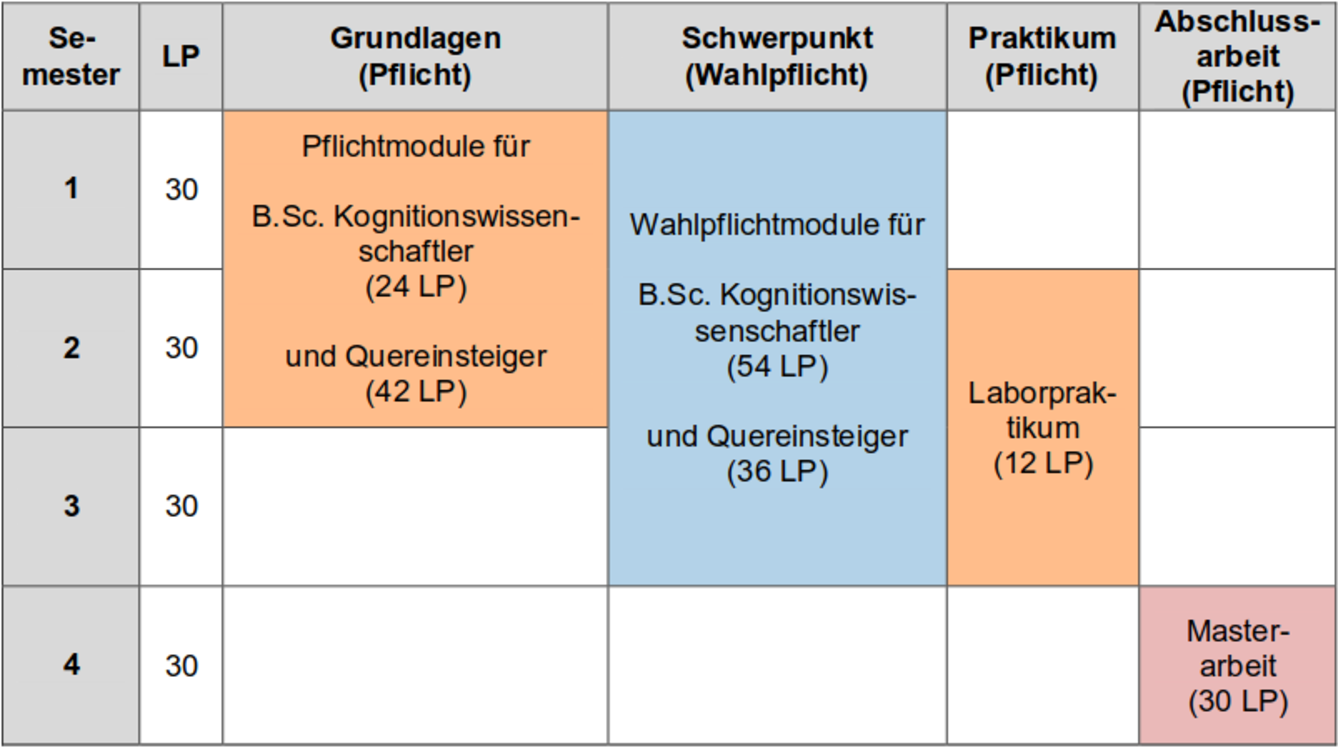
\includegraphics[width=.8\textwidth]{media/studienplan_kmsc.pdf}
\end{center}
%Genauere Informationen zu den einzelnen Modulen findet ihr im Modulhandbuch\\ (http://www.wsi.uni-tuebingen.de/studium/downloads/modulhandbuecher.html). \\
%\\
Zu beachten ist die Gewichtung der verschiedenen Module und die Reihenfolge, in der die Module mit Kursen aufgefüllt werden. Wenn
du z.B. das Modul MKOGINF mit Informatikkursen aufgefüllt hast, ist es unter Umständen schwierig, diese Kurse durch Kurse mit
besserer Note zu ersetzen. Nähere Informationen dazu werden euch bei der Einführungsveranstaltung zum Master Kognitionswissenschaft mitgeteilt. Ferner spielen im Master für einige Studierende Auflagen eine wichtige Rolle. In deinem Zulassungsbescheid bist du darüber informiert worden, ob du in der Psychologie und/oder Informatik Auflagen erfüllen musst. Dies bedeutet, dass du in dem jeweiligen Fach einige Grundveranstaltungen besuchen musst. Zu den Auflagen bekommst du ebenfalls bei der Einführungsveranstaltung genauere Informationen mitgeteilt. In seltenen Fällen können Auflagen gestrichen werden, falls im Bachelor vergleichbare Leistungen erbracht wurden. Hierfür kannst du dich an Frau Seibold wenden, die die Angelegenheit mit dem Studiendekan Prof. Wichmann abklärt (anerkennung\At kogwis.uni-tuebingen.de). Generell kannst du dich bei Fragen zur Studienorganisation ebenso bei Frau Seibold melden (studienberatung\At kogwis.uni-tuebingen.de). Exemplarische Studienpläne, abhängig von deinen Auflagen, kannst du auch im Modulhandbuch nachsehen, welches du hier findest: https://www.wsi.uni-tuebingen.de/studium/downloads/modulhandbuecher-und-veranstaltungsverzeichnisse.html.
\fi

\ifinfo
	\iflehramt
	\else
	Im Modulhandbuch für den Master in Informatik wird dieser Beispiel-Studienplan vorgeschlagen:
	\begin{center}
		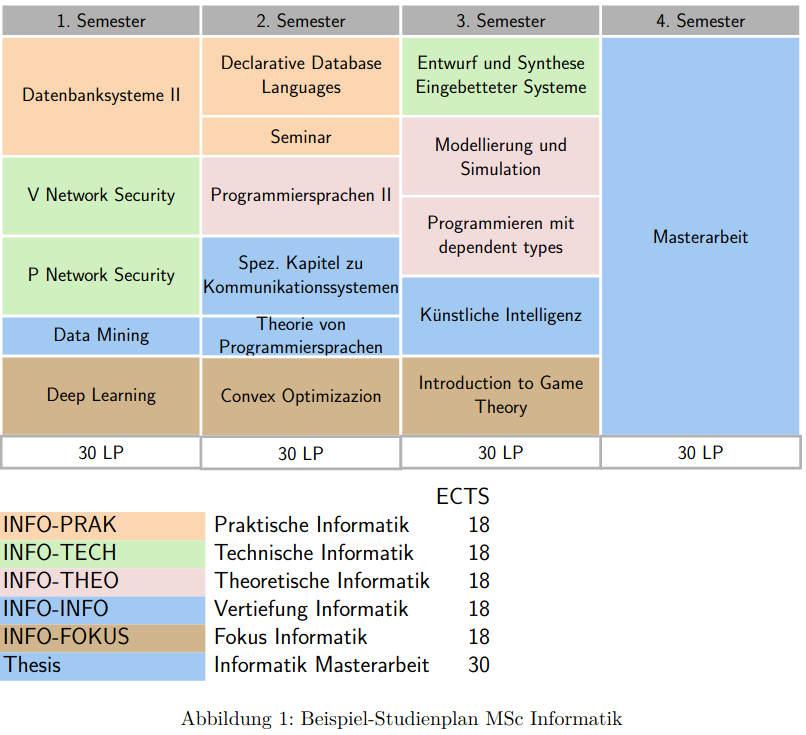
\includegraphics[width=0.8\textwidth]{media/studienplan_msc.png}
	\end{center}
	\newpage
	\fi
\fi
